\documentclass[10pt,showpacs,preprintnumbers,footinbib,amsmath,amssymb,aps,prl,twocolumn,groupedaddress,superscriptaddress,showkeys]{revtex4-1}
\usepackage{graphicx}
\usepackage{dcolumn}
\usepackage{bm}
\usepackage[colorlinks=true,urlcolor=blue,citecolor=blue]{hyperref}
\usepackage{color}
\usepackage{listings}
\usepackage{subfig}

\lstset{ %
  basicstyle=\footnotesize,        % the size of the fonts that are used for the code
  breakatwhitespace=false,         % sets if automatic breaks should only happen at whitespace
  breaklines=true,                 % sets automatic line breaking
  captionpos=t,                    % sets the caption-position to bottom
  deletekeywords={...},            % if you want to delete keywords from the given language
  escapeinside={\%*}{*)},          % if you want to add LaTeX within your code
  extendedchars=true,              % lets you use non-ASCII characters; for 8-bits encodings only, does not work with UTF-8
  frame=single,                    % adds a frame around the code
  keepspaces=true,                 % keeps spaces in text, useful for keeping indentation of code (possibly needs columns=flexible)
 % language=Python,                 % the language of the code
  morekeywords={*,...},           % if you want to add more keywords to the set
  numbers=left,                    % where to put the line-numbers; possible values are (none, left, right)
  numbersep=5pt,                   % how far the line-numbers are from the code
  showspaces=false,                % show spaces everywhere adding particular underscores; it overrides 'showstringspaces'
  showstringspaces=false,          % underline spaces within strings only
  showtabs=false,                  % show tabs within strings adding particular underscores
  stepnumber=1,                    % the step between two line-numbers. If it's 1, each line will be numbered
  tabsize=2,                       % sets default tabsize to 2 spaces
}


\begin{document}
\title{FYS3150 Computational Physics - Project 3}
\author{Nicholas Karlsen}

\begin{abstract}
This is an abstract
\end{abstract}

\maketitle

\section{Introduction}

  In this report we will take a look at two methods for solving Ordinary differential equations (ODE) numerically, which is of great interest to physicists, as a lot of physical systems are governed by such equations, most of which lack analytical solutions. In particular, 
  
  Lastly, the source code for any code discussed in this report can be found on my
  Github at: \url{https://github.com/nicholaskarlsen/FYS3150}

\section{Theory, Algorithms and Methods}
  
  \subsection{Newton's law of universal gravitation}
    Between every body, there is a force of attraction inversly proportional to the square of the separation, or more precisely, the force acting on some body with mass $m$ due to a mass $m'$ is
    \begin{equation}
      \mathbf F = -G\frac{m m'}{|\mathbf r - \mathbf r'|^2}\mathbf{\hat{u}_{r-r'}}, \quad \mathbf{\hat{u}_{r-r'}} = \frac{\mathbf r - \mathbf r'}{\mathbf |\mathbf r - \mathbf r'|}
    \end{equation}
    Where $G$ is the gravitational constant and $\mathbf r, \mathbf r'$ denote the position vectors of bodies with mass $m, m'$ respectively.

    Chosing the the 2D cartesian coordinate system, let $\mathbf r - \mathbf r'= (x_{r}, y_{r})$, where the $r$ suffix denote that these coordinates are to be understood as the relative coordinates between bodies $m, m'$.
    Further, $|\mathbf r - \mathbf r'| = \sqrt{x_r^2 + y_r^2} = r$ is the distance between the two bodies.

    By Newtons second law, the acceleration on body 1 due to the gravitational pull of body 2 can then be written as
    \begin{equation}
      \mathbf a = \frac{1}{m}\mathbf F = -G \frac{m'}{r^2}\frac{(\mathbf r-\mathbf r')}{r} = -G\frac{m'}{r^2}\frac{\left(x_r, y_r\right)}{r}
    \end{equation}
    Written out component-wise in terms of the positions, we get the set of coupled differential equations

    \begin{equation}
      \frac{\partial^2 x}{\partial t^2} = -G\frac{m'}{r^2}\frac{x_r}{r}, \quad
      \frac{\partial^2 y}{\partial t^2} = -G\frac{m'}{r^2}\frac{y_r}{r}
    \end{equation}
    Similar, for 3 dimensions where $\mathbf r - \mathbf r' = (x_r, y_r, z_r), r=\sqrt{x_r^2 + y_r^2 + z_r^2}$.

    \subsubsection{Relativistic Correction}

      \begin{figure}[h!]
        \center
        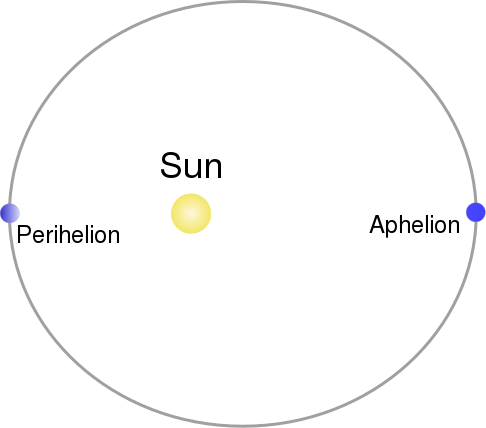
\includegraphics[width=4cm]{figs/486px-Perihelion-Aphelion.png}
        \caption{In an eliptic orbit, the closest and farthest points in the orbit is defined as the Perhelion and Aphelion respectively [\href{https://en.wikipedia.org/wiki/Perihelion_and_aphelion}{Image source}]}
        \label{fig:perhelion}
      \end{figure}

      The aforementioned model of gravity fails to predict the perihelion (see fig. \ref{fig:perhelion}) precession of mercury, which is observed to be $43"$ per century \cite{problem_set}. 

      That is, the closed, uniform elliptical orbits predicted by the Newtonian model for gravity does not match with observations in Astronomy, where the perihelion of Mercury seems to shift over time. In fact, the perihelion precession of mercury was the first experimental confirmations of General relativity, which accurately predicts this phenomena.

      And so, a correcting factor accounting for the relativistic effects is added to Newtons model, and the magnitude of the gravitational force becomes \cite{problem_set}

      \begin{equation}
        |\mathbf F| = G \frac{m m'}{r^2}\left[1 + \frac{3l^2}{r^2c^2}\right]
      \end{equation}
      Where $l$ denotes the magnitude of the angular momentum of the orbiting body and $c$ the speed of light.

      Now, in order to find the perihelion precession we define a coordinate system such that 

\subsection{Solving ODEs numerically}
  \subsubsection{Forward Euler}
    Consider a function $f(t)$, which derivative, $f'(t)$ is known and we want to find $f(t + \delta t)$. 
    Take the taylor expansion of $f(t + \delta t)$
    \begin{equation}
      f(t + \delta t) = f(t) + f'(t)\delta t + \frac{1}{2}f''(t)\delta t^2 + \dots + \frac{1}{n!}f^{(n)}(t)\delta t^n
    \end{equation}
    If we then truncate this series after the second term we get
    \begin{equation}
      f(t + \delta t) = f(t) + f'(t)\delta t + \mathcal O(\delta t^2)
    \end{equation}
    where the term $\mathcal O(\delta t^2)$ contains the numerical error associated by truncating the series early.

    Since $f(t), f'(t)$ are known, this allows us to find $f(t + \delta t)$, which is the basis of the Forward Euler algorithm. Following, i have written out in pseudocode how this algorithm can be used to solve a system governed by some known force $\mathbf F$ and initial conditions $\mathbf v(0) \simeq v_0, \mathbf r(0) \simeq r_0$.

    \begin{lstlisting}[mathescape=true, language=python, title=Forward Euler Algorithm]
  for $i = 0, \dots, N-1$
      $\mathbf v_{i + 1} = \mathbf v_{i} + \mathbf a_{i}\Delta t$
      $\mathbf r_{i + 1} = \mathbf r_{i} + \mathbf v_{i}\Delta t$
  \end{lstlisting}

  Notice that the value of $\mathbf v_{i+1}$ is known when computing $\mathbf r_{i+1}$. By using this newly calculated velocity in the computation instead, we get the Euler-Cromer method, which wont be discussed further in this report.

  \begin{lstlisting}[mathescape=true, language=python, title=Euler-Cromer Algorithm]
  for $i = 0, \dots, N-1$
      $\mathbf v_{i + 1} = \mathbf v_{i} + \mathbf a_{i}\Delta t$
      $\mathbf r_{i + 1} = \mathbf r_{i} + \mathbf v_{i + 1}\Delta t$
  \end{lstlisting}

  \subsubsection{Velocity-Verlet}
    The Velocity-Verlet method is another method for solving ODE's numerically, which just like Forward Euler is derived from the manipulation of Taylor expansions. However, this time i refer you to \cite{ode_lecture} for the full derivation and simply state the result

    \begin{align}
      \begin{split}
        f(t + \delta t) &= f(t) + f'(t)\delta t + \frac{f''(t)\delta t}{2} + \mathcal O(\delta t^3) \\
        f'(t + \delta t) &= f'(t) + \frac{\left( f''(t + \delta t) + f''(t) \right)\delta t}{2} + \mathcal O(\delta t^3)
      \end{split}
    \end{align}
    Which again, can be applied to solve a Physical system where $\mathbf F$ is known. The algorithm for doing this is written out below
  \begin{lstlisting}[mathescape=true, language=python, title=Velocity-Verlet Algorithm]
  for $i = 0, \dots, N-1$
    $\mathbf r_{i+1} = \mathbf r_i + \mathbf v_i \Delta t + \frac{1}{2}\mathbf a_i(\Delta t)^2$
    $\mathbf v_{i+1} = \mathbf v_i + \frac{1}{2}(\mathbf a_{i+1} + \mathbf a_i)\Delta t  $
  \end{lstlisting}



\section{Results and Discussions}
  \subsection{Object orientation}
    When designing the class \lstinline{n_solver}, i wanted to strike a balance between utilizing the benefits, and expandability you get from object orientation whilst also not abstracting the data too much. As such, the class simply manipulates arrays of a particular format in a particular way. Not abstracting the process by creating objects for each planet (or something else of that nature), which seems to be a pitfall of object orientation as i perceive it.

    As such, the class can easily be expanded by adding new solvers and differential equations, to solve similar multi-body problems governed by a different set of coupled differential equations.

    A particular benefit in the way i wrote my code, is that there is no difference if the input data is in 2 Dimensions or 3. The code will work just the same either way by making full use of the way Numpy arrays work.

    I also made an attempt to utilize just-in-time (JIT) compilation by using jitclass from the Numba package, however, jitclass is poorly documented in its current state and imposes many restrictions as to what is permitted compared to regular python, or even the standard jit flag that is used for regular python functions. Eventually, i reached the point where i would have to sacrifice the modularity of my program in order to run it using jitclass, which obviously was not an option. So i gave up on the endeavor.

  \subsection{Earth-Sun System}

    Working in units $M_\odot, AU, Years$ for mass, length and time respectively, i initialized a 2D system using the \lstinline{n_solver} class where the sun is fixed at the origin and the earth has initial velocity $\mathbf v_0 = (0, 2\pi)$ at position $\mathbf r_0 = (1, 0)$, corresponding to an orbit of eccentricity, $e=0$, a perfect circle.
    
    \begin{figure}
      \center
      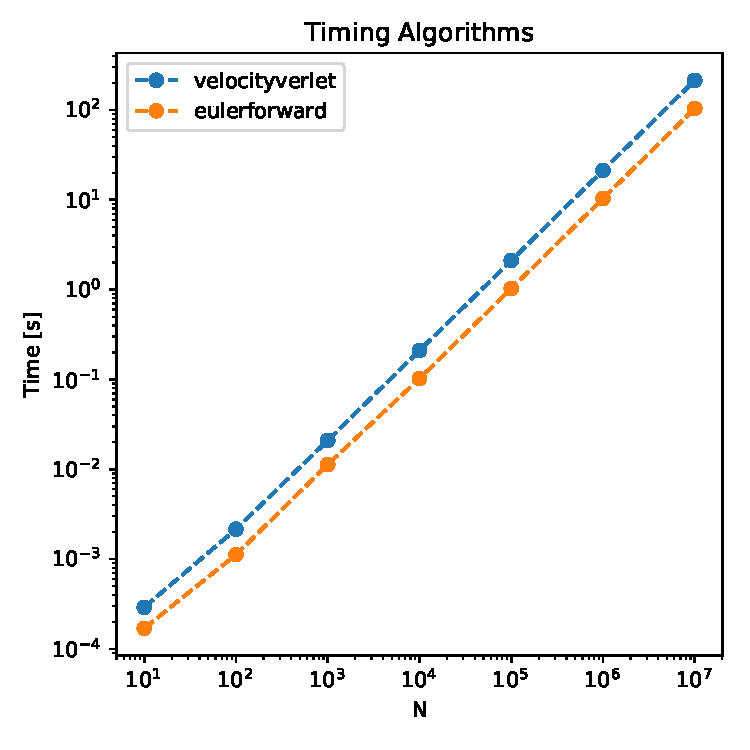
\includegraphics[width=8cm]{figs/timing_earthsun.pdf}
      \caption{Time taken to solve the Earth-Sun system for different number of integration points for $t_n=10\, Yr$}
      \label{fig:timing}
    \end{figure}

    The system was then simulated for a time period of $10$ years using a different number of integration points for both the Velocity-Verlet and Forward Euler algorithms. The resulting orbits shown in Fig. \ref{fig:3c_earthsun}, shows that the Velocity-Verlet solution yields a reasonable approximate orbit for $N=10^3$ integration points, whilst the Forward Euler algorithm doesn't produce a comparable orbit until $N=10^6$ integration points. In Fig. \ref{fig:timing} we see the time it took for my program to solve this system for a selection of $N$. These numbers apply of course, only to the system with a fixed sun with one planet orbiting, as calculating the acceleration on more than one planets adds to the number of FLOPS.

    In Figures \ref{fig:c_speed}, \ref{fig:c_radius} we see how the speed and radius evolves throughout the integration points for $N=10^6$, and most notably, how they change. As mentioned prior, for the set of initial conditions used, we expect a perfectly circular orbit, but also constant speed. Looking at Figures \ref{fig:earthsun speed forward euler}, \ref{fig:c_radius_euler}, corresponding to the Forward Euler solution, that the earth is slightly drifting away from the sun, whilst loosing speed, which further implies that both the potential and kinetic energy in the system has not been conserved. Now we turn to Figures \ref{fig:earthsun speed verlet}, \ref{fig:c_radius_verlet}, corresponding to the Velocity-Verlet solution, where we see a periodic, but seemingly constant behavior of both the radius and speed, meaning that on average the energy of the system is conserved. Since the angular momentum is proportional to the product of the speed and radius, it follows that it is conserved and not conserved for the Verlet and Euler algorithms respectively.

\begin{figure*}[h!p]
  \center
  \subfloat[][Velocity-Verlet]{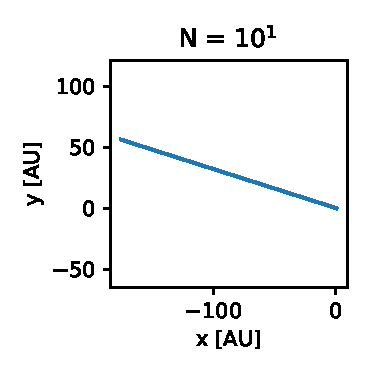
\includegraphics[width=4cm]{figs/ex_b_orbit_velocityverlet_1.pdf}}
  \subfloat[][Forward Euler]{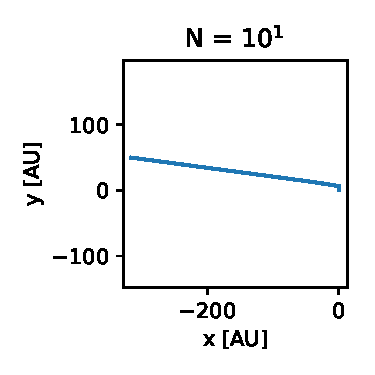
\includegraphics[width=4cm]{figs/ex_b_orbit_eulerforward_1.pdf}} 
  \subfloat[][Velocity-Verlet]{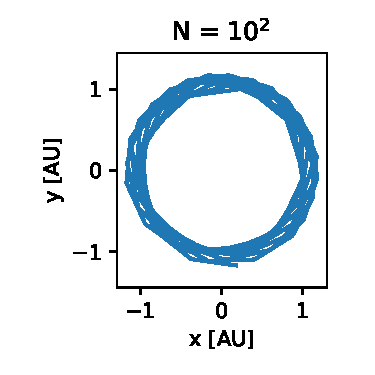
\includegraphics[width=4cm]{figs/ex_b_orbit_velocityverlet_2.pdf}}
  \subfloat[][Forward Euler]{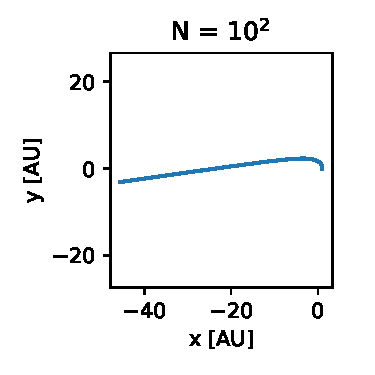
\includegraphics[width=4cm]{figs/ex_b_orbit_eulerforward_2.pdf}} 
  \\
  \subfloat[][Velocity-Verlet]{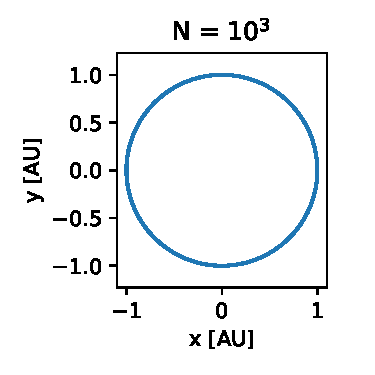
\includegraphics[width=4cm]{figs/ex_b_orbit_velocityverlet_3.pdf}}
  \subfloat[][Forward Euler]{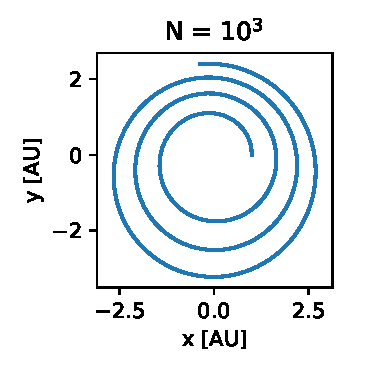
\includegraphics[width=4cm]{figs/ex_b_orbit_eulerforward_3.pdf}} 
  \subfloat[][Velocity-Verlet]{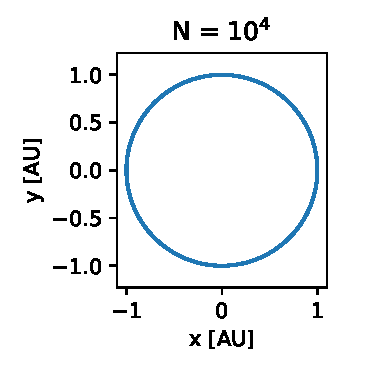
\includegraphics[width=4cm]{figs/ex_b_orbit_velocityverlet_4.pdf}}
  \subfloat[][Forward Euler]{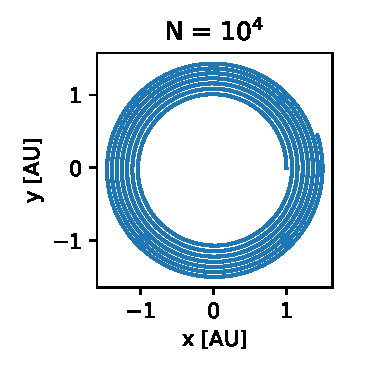
\includegraphics[width=4cm]{figs/ex_b_orbit_eulerforward_4.pdf}} 
  \\
  \subfloat[][Velocity-Verlet]{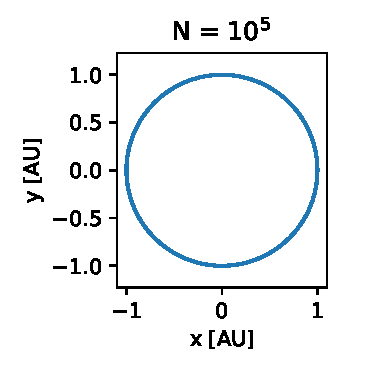
\includegraphics[width=4cm]{figs/ex_b_orbit_velocityverlet_5.pdf}}
  \subfloat[][Forward Euler]{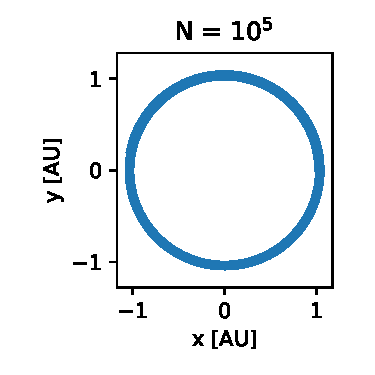
\includegraphics[width=4cm]{figs/ex_b_orbit_eulerforward_5.pdf}}
  \subfloat[][Velocity-Verlet]{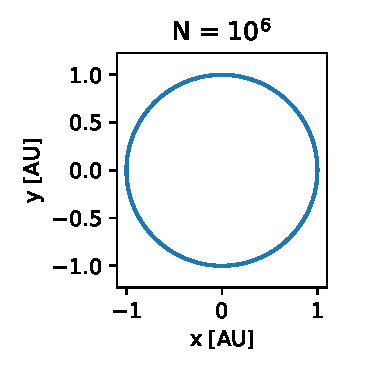
\includegraphics[width=4cm]{figs/ex_b_orbit_velocityverlet_6.pdf}}
  \subfloat[][Forward Euler]{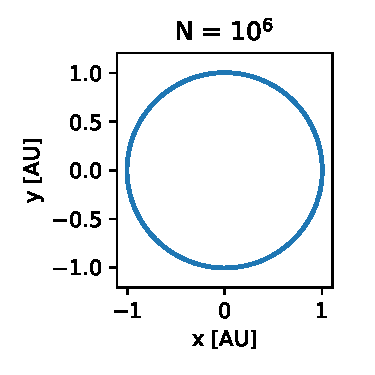
\includegraphics[width=4cm]{figs/ex_b_orbit_eulerforward_6.pdf}} 
  \caption{The orbit of earth around a stationary sun for a timeperiod of 10 Years with simulated with a varying number of integration points N (see fig titles) using the Velocity-Verlet and Forward Euler algorithms}
  \label{fig:3c_earthsun}
\end{figure*}
 
\begin{figure*}
  \center
  \subfloat[][Velocity-Verlet]{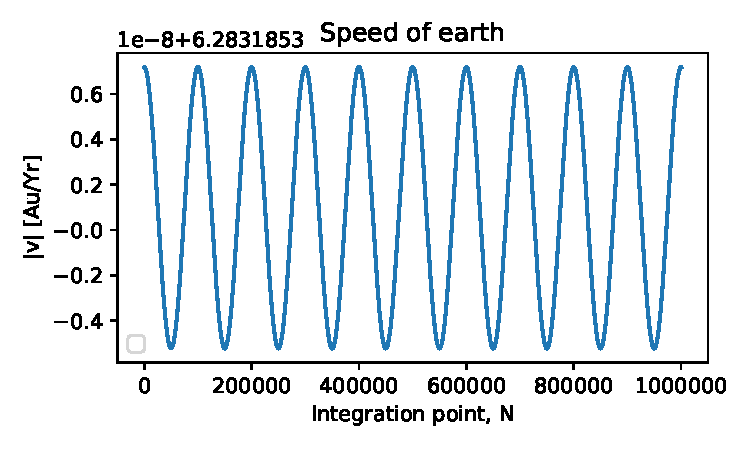
\includegraphics[width=8cm]{figs/ex_b_speed_velocityverlet_6.pdf}\label{fig:earthsun speed verlet}}
   \subfloat[][Forward Euler]{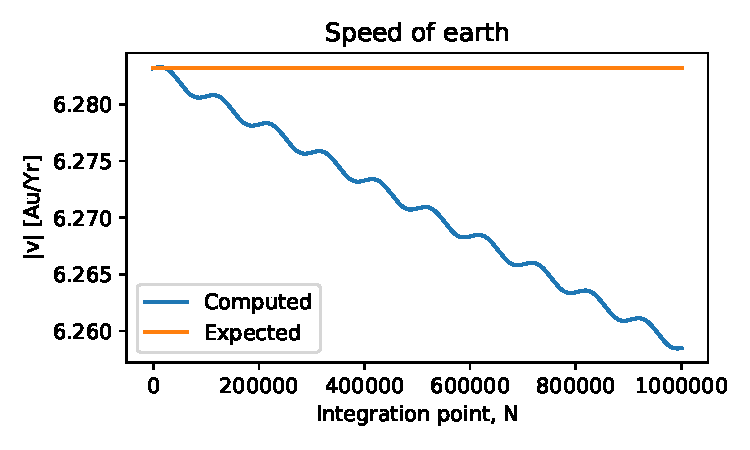
\includegraphics[width=8cm]{figs/ex_b_speed_eulerforward_6.pdf}\label{fig:earthsun speed forward euler}}
   \caption{The speed of Earth in the Earth-Sun system for solutions using the Velocity-Verlet algorithm (a) and the Forward Euler algorithm (b) in a 10 Year simulation and $N=10^6$ integration points}
   \label{fig:c_speed}
\end{figure*}
\begin{figure*}
  \center
  \subfloat[][Velocity-Verlet]{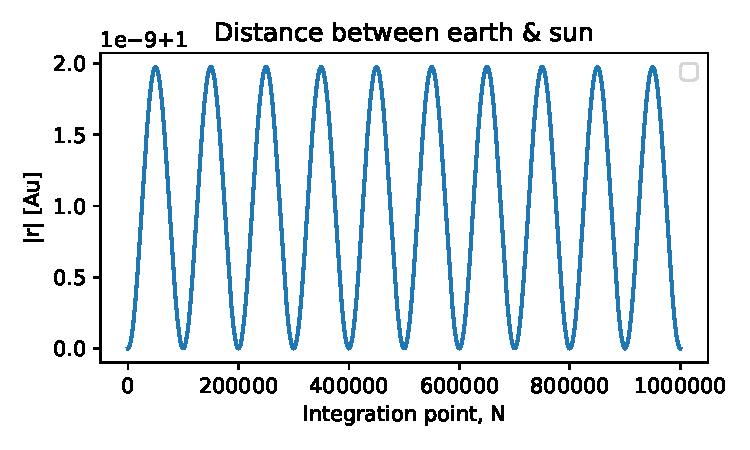
\includegraphics[width=8cm]{figs/ex_b_radius_velocityverlet_6.pdf}\label{fig:earthsun potential verlet}\label{fig:c_radius_verlet}}
   \subfloat[][Forward Euler]{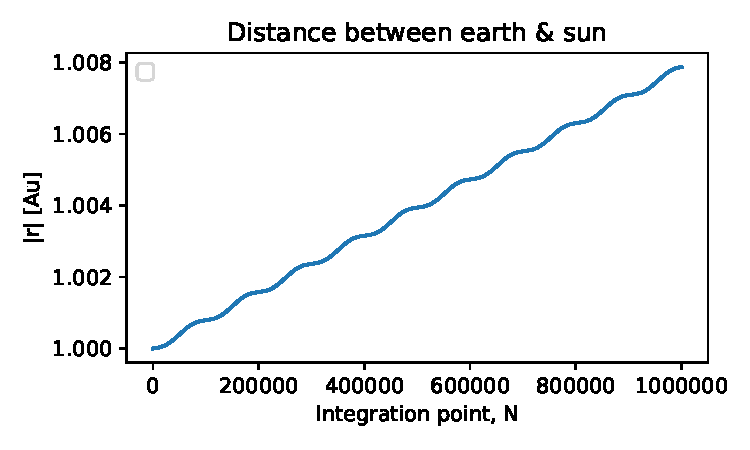
\includegraphics[width=8cm]{figs/ex_b_radius_eulerforward_6.pdf}\label{fig:earthsun potential forwardeuler}\label{fig:c_radius_euler}}
   \caption{The radius of Earth in the Earth-Sun system for solutions using the Velocity-Verlet algorithm (a) and the Forward Euler algorithm (b) in a 10 Year simulation and $N=10^6$ integration points}
   \label{fig:c_radius}
\end{figure*}


\begin{figure*}
  \center
  \subfloat[][]{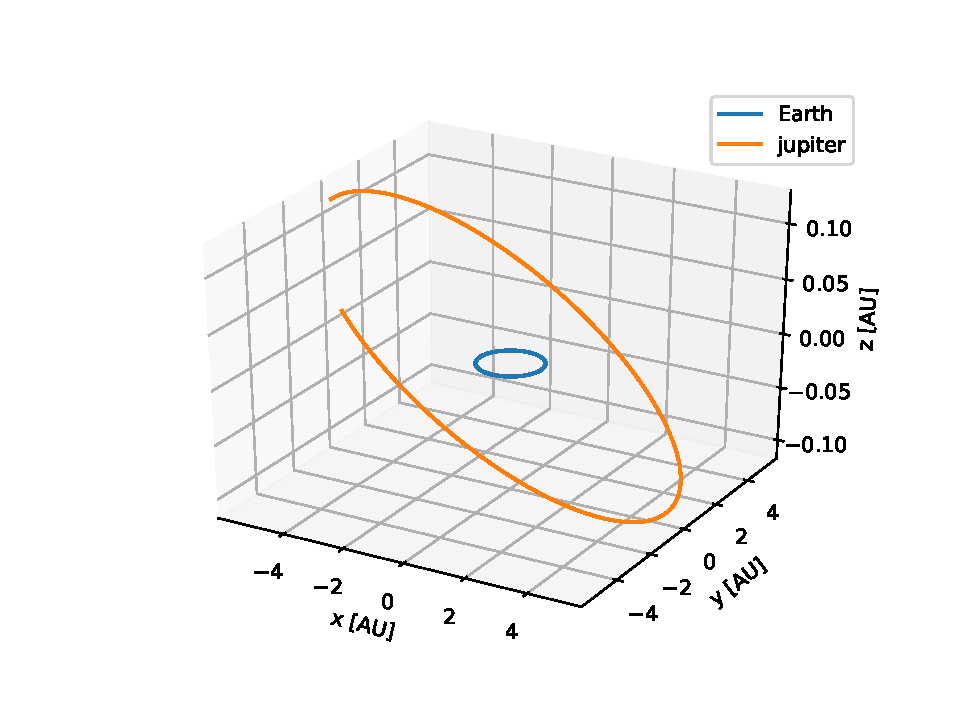
\includegraphics[width=14cm]{figs/exe_earth_jupiter_10.pdf}}\\
  \subfloat[][]{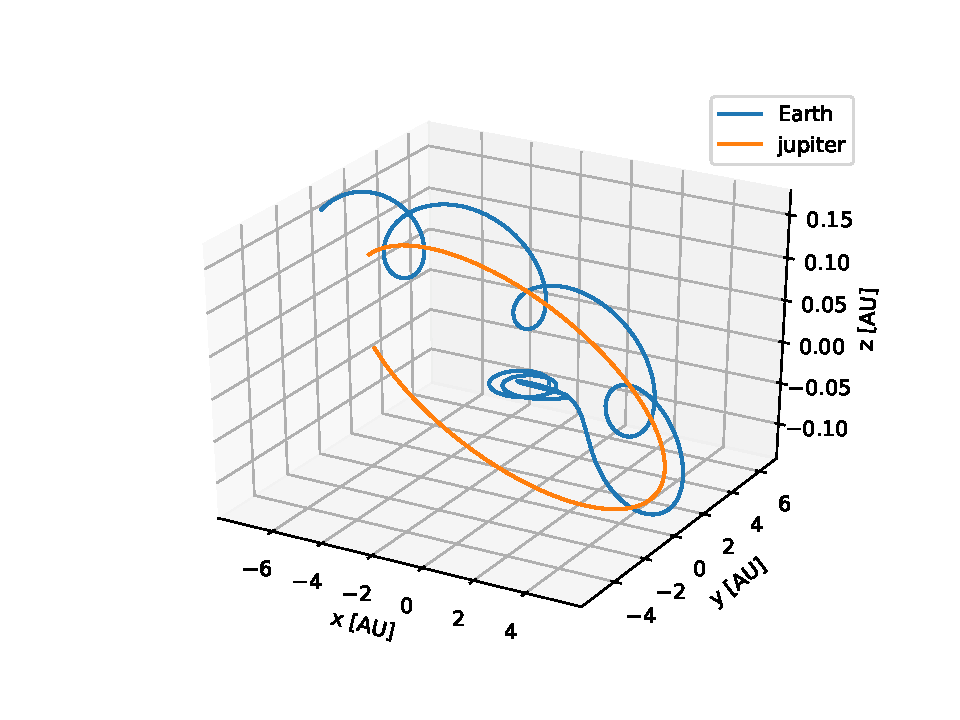
\includegraphics[width=14cm]{figs/exe_earth_jupiter_1000.pdf}}
\end{figure*}

\begin{figure}
  \center
  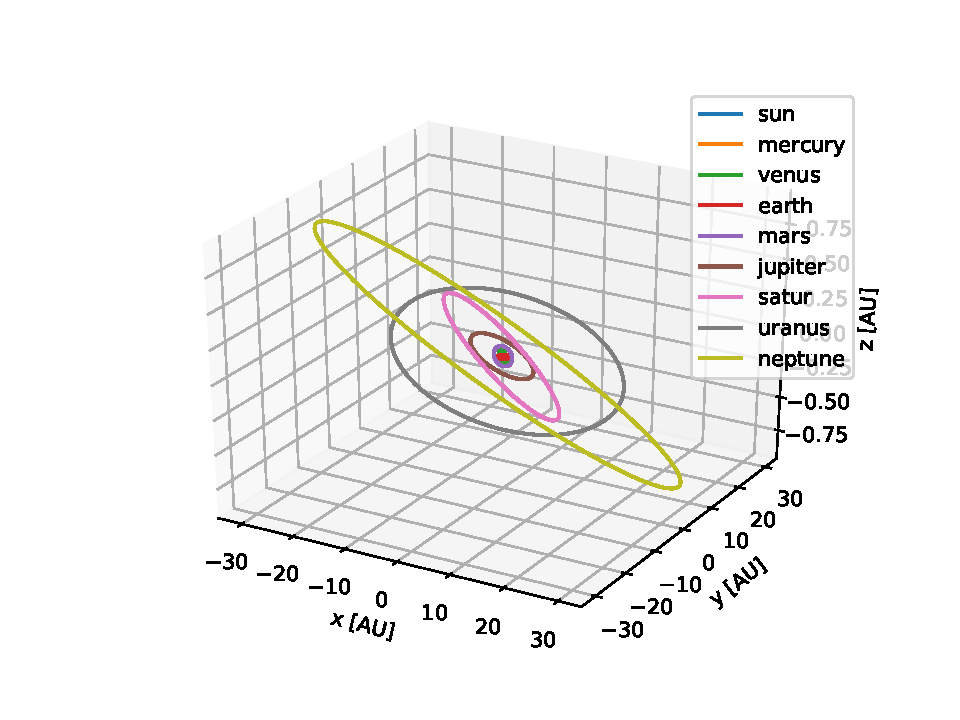
\includegraphics{figs/all_planets3d.pdf}
\end{figure}




\section{Conclusions}


\begin{thebibliography}{99}
\bibitem{lecture_notes} M.~Hjorth-Jensen, Computational Physics - Lecture Notes 2015, (2015).
\bibitem{ode_lecture} M.~Hjorth-Jensen, Ordinary differential equations - Computational Physics Lectures (2017)
\bibitem{problem_set} M.~Hjorth-Jensen, Building a model for the solar system using ordinary differ-
ential equations - Project 3 (2018)
\end{thebibliography}



\end{document}  